\section{Results}

We organize the results around two empirically separable stages of revision behavior: the revision gate (whether the model revises) and intensity calibration (how much it overcorrects). We present evidence for each stage in turn.

\subsection{RQ1: The Revision Gate}

The follow-up probe dominates the revision gate; the stated quality threshold has no detectable effect. Under the leading probe (``Can this be improved?''), models revised in 99.9\% of trials: Claude Sonnet 4 and GPT-4o declined 0.0\% of the time, and Gemini 2.5 Flash declined just 0.2\%. Under the evaluative probe, decline rates diverged sharply by model (see RQ3 below), but across all models the revision rate dropped to a mean of 23.2\%.

Chi-squared tests confirm that the revision gate distribution differs significantly by probe type (Claude: $\chi^2 = 914.37$, $p < 0.0001$; Gemini: $\chi^2 = 1326.89$, $p < 0.0001$; GPT-4o: $\chi^2 = 788.96$, $p < 0.0001$).\footnote{These chi-squared tests include all five pilot probe types, not just the two main probes; degrees of freedom reflect the full 5-probe $\times$ 3-category contingency table.} The quality threshold, by contrast, does not significantly affect the revision gate distribution for any model (Kruskal-Wallis $p > 0.40$ for all models). Given the study's power to detect proportion differences as small as 0.032, these null results are unlikely to reflect insufficient power. The full gate distribution by model and probe type is shown in the appendix.

In the ordinal regression (Model A), the leading probe is by far the strongest predictor of overcorrection ($\beta = 3.47$, $z = 33.73$, $p < 0.001$), dwarfing all other coefficients (Table~\ref{tab:regression}). This effect strengthens when scenario fixed effects are added (Model B: $\beta = 3.94$, $p < 0.001$). Adding a probe $\times$ threshold interaction term yields a significant coefficient ($\beta = -2.20$, $z = -5.69$, $p < 0.001$), but this result is consistent with a floor effect: the evaluative probe suppresses revision almost entirely, leaving minimal overcorrection variance for the threshold to modulate. The threshold effect is concentrated in the leading-probe condition (net slope $= -1.40$), while the evaluative-probe slope ($+0.80$) is driven by the small minority of trials that pass the gate.

\begin{table}[t]
\centering
\small
\begin{tabular}{@{}lrrr@{}}
\toprule
\textbf{Predictor} & \textbf{Model A} & \textbf{Model B} & \textbf{Model C} \\
\midrule
is\_leading & $3.47^{***}$ & $3.94^{***}$ & --- \\
threshold & $-0.93^{***}$ & $-1.04^{***}$ & $-1.65^{***}$ \\
is\_qualitative & $-0.74^{***}$ & $-0.85^{***}$ & $-1.05^{***}$ \\
Claude Sonnet & $0.10$ & $0.15$ & $0.33^{**}$ \\
Gemini Flash & $0.42^{***}$ & $0.52^{***}$ & $1.15^{***}$ \\
Scenario FEs & No & Yes & Yes \\
\midrule
$N$ & 3,840 & 3,840 & 1,920 \\
AIC & 5,319 & 4,839 & 3,545 \\
\bottomrule
\end{tabular}
\caption{Ordinal regression coefficients (overcorrection $\sim$ predictors). Model C is restricted to leading-probe trials. Threshold is scaled 0--1 (so $\beta = -1.65$ corresponds to the full range from no threshold to threshold 100). $^{**}p<0.01$, $^{***}p<0.001$. Reference model: GPT-4o.}
\label{tab:regression}
\end{table}

\subsection{RQ2: Threshold Sensitivity Within Revisions}

Within the leading-probe condition, where revision is universal, higher stated thresholds are associated with lower overcorrection scores, but the effect size varies substantially across models (Figure~\ref{fig:threshold-ladder}). Median overcorrection is 1.0 across all conditions, indicating that most individual trials show proportionate revision; the regression effects below are driven by a substantial minority of trials with moderate-to-severe overcorrection, concentrated in formal and creative writing scenarios (see Appendix Figure~\ref{fig:scenario-boxplots}).

\begin{figure*}[t]
    \centering
    
\includegraphics[width=\textwidth]{figures/02_threshold_ladder.pdf}
    \caption{Overcorrection by threshold level within leading-probe trials, one panel per model. Dashed line marks proportionate revision.}
    \label{fig:threshold-ladder}
\end{figure*}

Spearman correlations between threshold level and overcorrection (leading probe only) are:
\begin{itemize}
    \item Gemini 2.5 Flash: $\rho = -0.50$ ($p < 0.001$), moderate
    \item Claude Sonnet 4: $\rho = -0.35$ ($p < 0.001$), weak-to-moderate
    \item GPT-4o: $\rho = -0.14$ ($p < 0.001$), negligible-to-weak
\end{itemize}

Kruskal-Wallis $H$ tests across threshold levels confirm a significant threshold effect for Gemini (numeric: $H = 50.40$, $p < 0.0001$; qualitative: $H = 23.42$, $p = 0.001$) and Claude (numeric: $H = 17.59$, $p = 0.014$; qualitative: $H = 23.30$, $p = 0.002$), but not for GPT-4o (numeric: $H = 3.20$, $p = 0.87$; qualitative: $H = 4.89$, $p = 0.67$).

The ordinal regression restricted to leading-probe trials (Model C) confirms that threshold is a significant predictor after controlling for framing, model, and scenario ($\beta = -1.65$, $p < 0.001$). However, this coefficient is driven primarily by Gemini and Claude; GPT-4o shows negligible threshold sensitivity.

\subsection{RQ3: Model Differences in Revision Disposition}

Under the leading probe, all three models behave nearly identically ($\sim$100\% revision). The evaluative probe reveals sharply different revision dispositions:
\begin{itemize}
    \item Gemini 2.5 Flash: 99.7\% decline rate (almost never revises)
    \item GPT-4o: 68.6\% decline rate
    \item Claude Sonnet 4: 62.0\% decline rate (most willing to revise)
\end{itemize}

This divergence is consistent with the ordinal regression results: Gemini shows the strongest overcorrection tendency (Model C: $\beta = 1.15$, $p < 0.001$) but also the highest evaluative-probe decline rate. Gemini thus shows the most extreme combination: highest overcorrection when revising, highest decline rate when not. Claude and GPT-4o show more intermediate behavior across both probe conditions (Appendix Figure~\ref{fig:probe-cliff-model}).

\subsection{Framing Effects}

Qualitative threshold framings produce significantly less overcorrection than numeric framings (Model A: $\beta = -0.74$, $p < 0.001$; Model C: $\beta = -1.05$, $p < 0.001$). This effect is consistent across all three regression models and is not an artifact of scenario or model differences. Revision gate distributions do not differ by framing ($\chi^2$ tests: all $p > 0.77$), confirming that the framing effect operates at Stage 2 (intensity), not Stage 1 (gate). For the full framing comparison, see Appendix Figure~\ref{fig:framing-comparison}.

\subsection{Study 2: Momentum}

Study~2 tests whether prior revision rounds shift the revision gate on a subsequent evaluative probe. In the no-momentum baseline (dose $= 0$), the model receives only the scenario prompt and then the evaluative probe, with no prior revision requests; these trials are drawn from Study~1's evaluative-probe condition. In the momentum conditions (dose $= 1, 2, 3$), the model first completes one, two, or three rounds of ``Can this be improved?'' followed by revision before encountering the same evaluative probe.

\subsubsection{RQ4: Does Revision History Shift the Gate?}

Overall, revision history nearly doubles the evaluative-probe revision rate. Without any prior revision rounds, models revised 23.2\% of the time ($n = 1{,}920$); after 1--3 prior revision rounds, this rises to 44.6\% ($n = 1{,}813$). The gate distribution shift is highly significant ($\chi^2 = 376.54$, $p < 0.0001$, $df = 2$).

However, this aggregate effect masks dramatic model-level divergence (Table~\ref{tab:momentum-model}).

\begin{table}[t]
\centering
\small
\begin{tabular}{@{}lcccc@{}}
\toprule
\textbf{Model} & \textbf{Dose 0} & \textbf{Dose 1} & \textbf{Dose 2} & \textbf{Dose 3} \\
\midrule
GPT-4o & 31.4\% & 98.4\% & 99.5\% & 97.4\% \\
Claude Sonnet 4 & 38.0\% & 38.0\% & 27.1\% & 24.5\% \\
Gemini 2.5 Flash & 0.3\% & 12.8\% & 9.9\% & 8.6\% \\
\bottomrule
\end{tabular}
\caption{Revision rate at the evaluative probe by momentum dose and model. GPT-4o exhibits near-total sycophantic shift; Claude and Gemini resist or decline.}
\label{tab:momentum-model}
\end{table}

GPT-4o's revision rate jumps from 31.4\% to 98.4\% with a single prior revision round, reaching a ceiling that additional doses do not increase. Claude Sonnet 4 shows no positive momentum effect and actually \textit{declines} from 38.0\% to 24.5\% at dose~3. Gemini 2.5 Flash rises from its near-zero baseline (0.3\%) to a modest 12.8\% at dose~1, but does not increase further.

\subsubsection{RQ5: Dose-Response}

Across all models, the Spearman correlation between dose and revision (binary) is $\rho = 0.199$ ($p < 0.0001$). The significant but modest effect size reflects the step-function shape: the entire shift occurs between dose~0 and dose~1, with no additional gain at doses~2 and~3. The full revision rate (as opposed to any revision) follows the same pattern: 3.0\% at dose~0, jumping to 22.1\% at dose~1, with no further increase (Figure~\ref{fig:dose-response}).

\begin{figure}[t]
    \centering
    
\includegraphics[width=\columnwidth]{figures/dose_response_curve.pdf}
    \caption{Revision rate at the evaluative probe by momentum dose, per model. The momentum effect is a step function driven almost entirely by GPT-4o.}
    \label{fig:dose-response}
\end{figure}

\subsubsection{RQ6: Threshold $\times$ Momentum}

Logistic regression (revised $\sim$ dose $+$ threshold $+$ dose $\times$ threshold) confirms that dose is a significant predictor ($\beta = 0.28$, $z = 4.21$, $p < 0.0001$), but threshold level is not ($\beta = -0.001$, $p = 0.39$), and the interaction term is not significant ($\beta = 0.001$, $p = 0.51$). Momentum operates independently of the stated quality threshold, consistent with Study~1's finding that thresholds do not modulate the gate.

\subsubsection{Overcorrection Under Momentum}

Overcorrection scores increase modestly with dose (mean: 1.09 at dose~0 to 1.33 at dose~3; Kruskal-Wallis $H = 213.76$, $p < 0.0001$). However, medians remain at 1.0 across all doses, indicating that most trials show proportionate revision even under momentum. The effect is concentrated in GPT-4o trials, where the high revision rate at dose~1+ produces more opportunities for overcorrection.

\subsubsection{Reverse Momentum}

To test whether conversational framing can suppress revision below the no-momentum baseline, we ran a reverse condition (dose $= -1$) in which the model receives one round of affirming feedback (``This looks great, no changes needed'') before the evaluative probe. Across 576 scored trials, no model produced a full revision; all responses were either declines or minor suggestions:

\begin{itemize}
    \item Gemini 2.5 Flash: 0.0\% revision (down from 0.3\% at dose~0)
    \item GPT-4o: 1.0\% revision (down from 31.4\% at dose~0)
    \item Claude Sonnet 4: 21.9\% revision (down from 38.0\% at dose~0), all minor suggestions
\end{itemize}

GPT-4o's trajectory illustrates the range of the framing effect: affirming feedback drops revision from 31.4\% to 1.0\%, while a single round of revision-prompting feedback raises it to 98.4\%. Claude shows the most resistance to suppression, still offering minor suggestions in about one-fifth of trials, consistent with its tendency to provide feedback even when not asked. No model produced a full revision under reverse momentum.

\subsection{Robustness}
\label{sec:robustness}

\paragraph{Length Proxy.} Response length delta (Turn 2 $-$ Turn 1 character count) serves as a judge-independent proxy for overcorrection. Spearman correlations between length delta and judge overcorrection scores are positive and significant for Claude ($\rho = 0.20$, $p < 0.001$) and Gemini ($\rho = 0.56$, $p < 0.001$). GPT-4o shows a near-zero negative correlation ($\rho = -0.07$, $p = 0.008$), likely because GPT-4o's revisions are more editorial than expansive, reducing the utility of length as a proxy for this model. Between-model rankings on length delta are broadly consistent with judge rankings on overcorrection: Gemini shows the largest length increases, Claude intermediate, and GPT-4o the smallest.

\paragraph{Judge Self-Preferencing.} GPT-4o as judge does not significantly favor its own outputs on our primary dependent variable (overcorrection) after FDR correction ($p = 0.032 \to q = 0.055$). This result is borderline; we note it transparently rather than treating it as a clean null. On revision value, the judge scores GPT-4o outputs \textit{lower} than other models (self mean $= 1.84$ vs.\ other mean $= 2.27$), suggesting a conservative rather than self-preferencing bias. See Appendix Figure~\ref{fig:judge-bias} for the full comparison.

\paragraph{Context Length Confound.} A potential concern is that momentum trials have longer conversation histories, and that context length itself drives revision behavior. We test this by correlating context length with revision outcomes. The correlation between threshold level and response length delta is $r = 0.015$, effectively zero, confirming that threshold conditions do not systematically differ in length. Within momentum trials, longer contexts actually predict \textit{less} revision, not more: the relationship runs opposite to what a length confound would predict. Response length rankings across models (Gemini $>$ Claude $>$ GPT-4o) are consistent with judge-based overcorrection rankings, providing convergent validity.

\paragraph{Power.} Post-hoc power analysis confirms the study is massively overpowered for RQ1 (MDE for proportion difference $= 0.032$; observed $\approx 0.75$) and well-powered for RQ2 (MDE for $|\rho| = 0.064$; observed $0.14$--$0.50$).

\subsection{Study 3: Revision Yield}

Studies~1 and~2 show that the revision gate is phrasing-sensitive and that conversational momentum can shift it. Study~3 asks the downstream question: when a model is offered a balanced revision opportunity at every turn across five turns, what happens to output quality?

\subsubsection{Quality Degrades With Revision}
\label{sec:quality-degrades}

Mean quality drops monotonically from 4.34 at Turn~1 to 2.45 at Turn~5 in the revision-only pool (Figure~\ref{fig:revision-yield}). The sharpest decline occurs between Turns~1 and~2 ($\Delta = -1.11$), with continued degradation at each subsequent turn. By Turn~5, the mean quality level has fallen below ``Incomplete'' on the six-level scale.

The decline rate by turn shows a complementary pattern: 31.8\% of models decline to revise at Turn~2, rising to 64.9\% by Turn~5. Even the balanced probe, which explicitly offers an off-ramp, fails to prevent the majority of models from revising when revision degrades quality.

\begin{figure}[t]
    \centering
    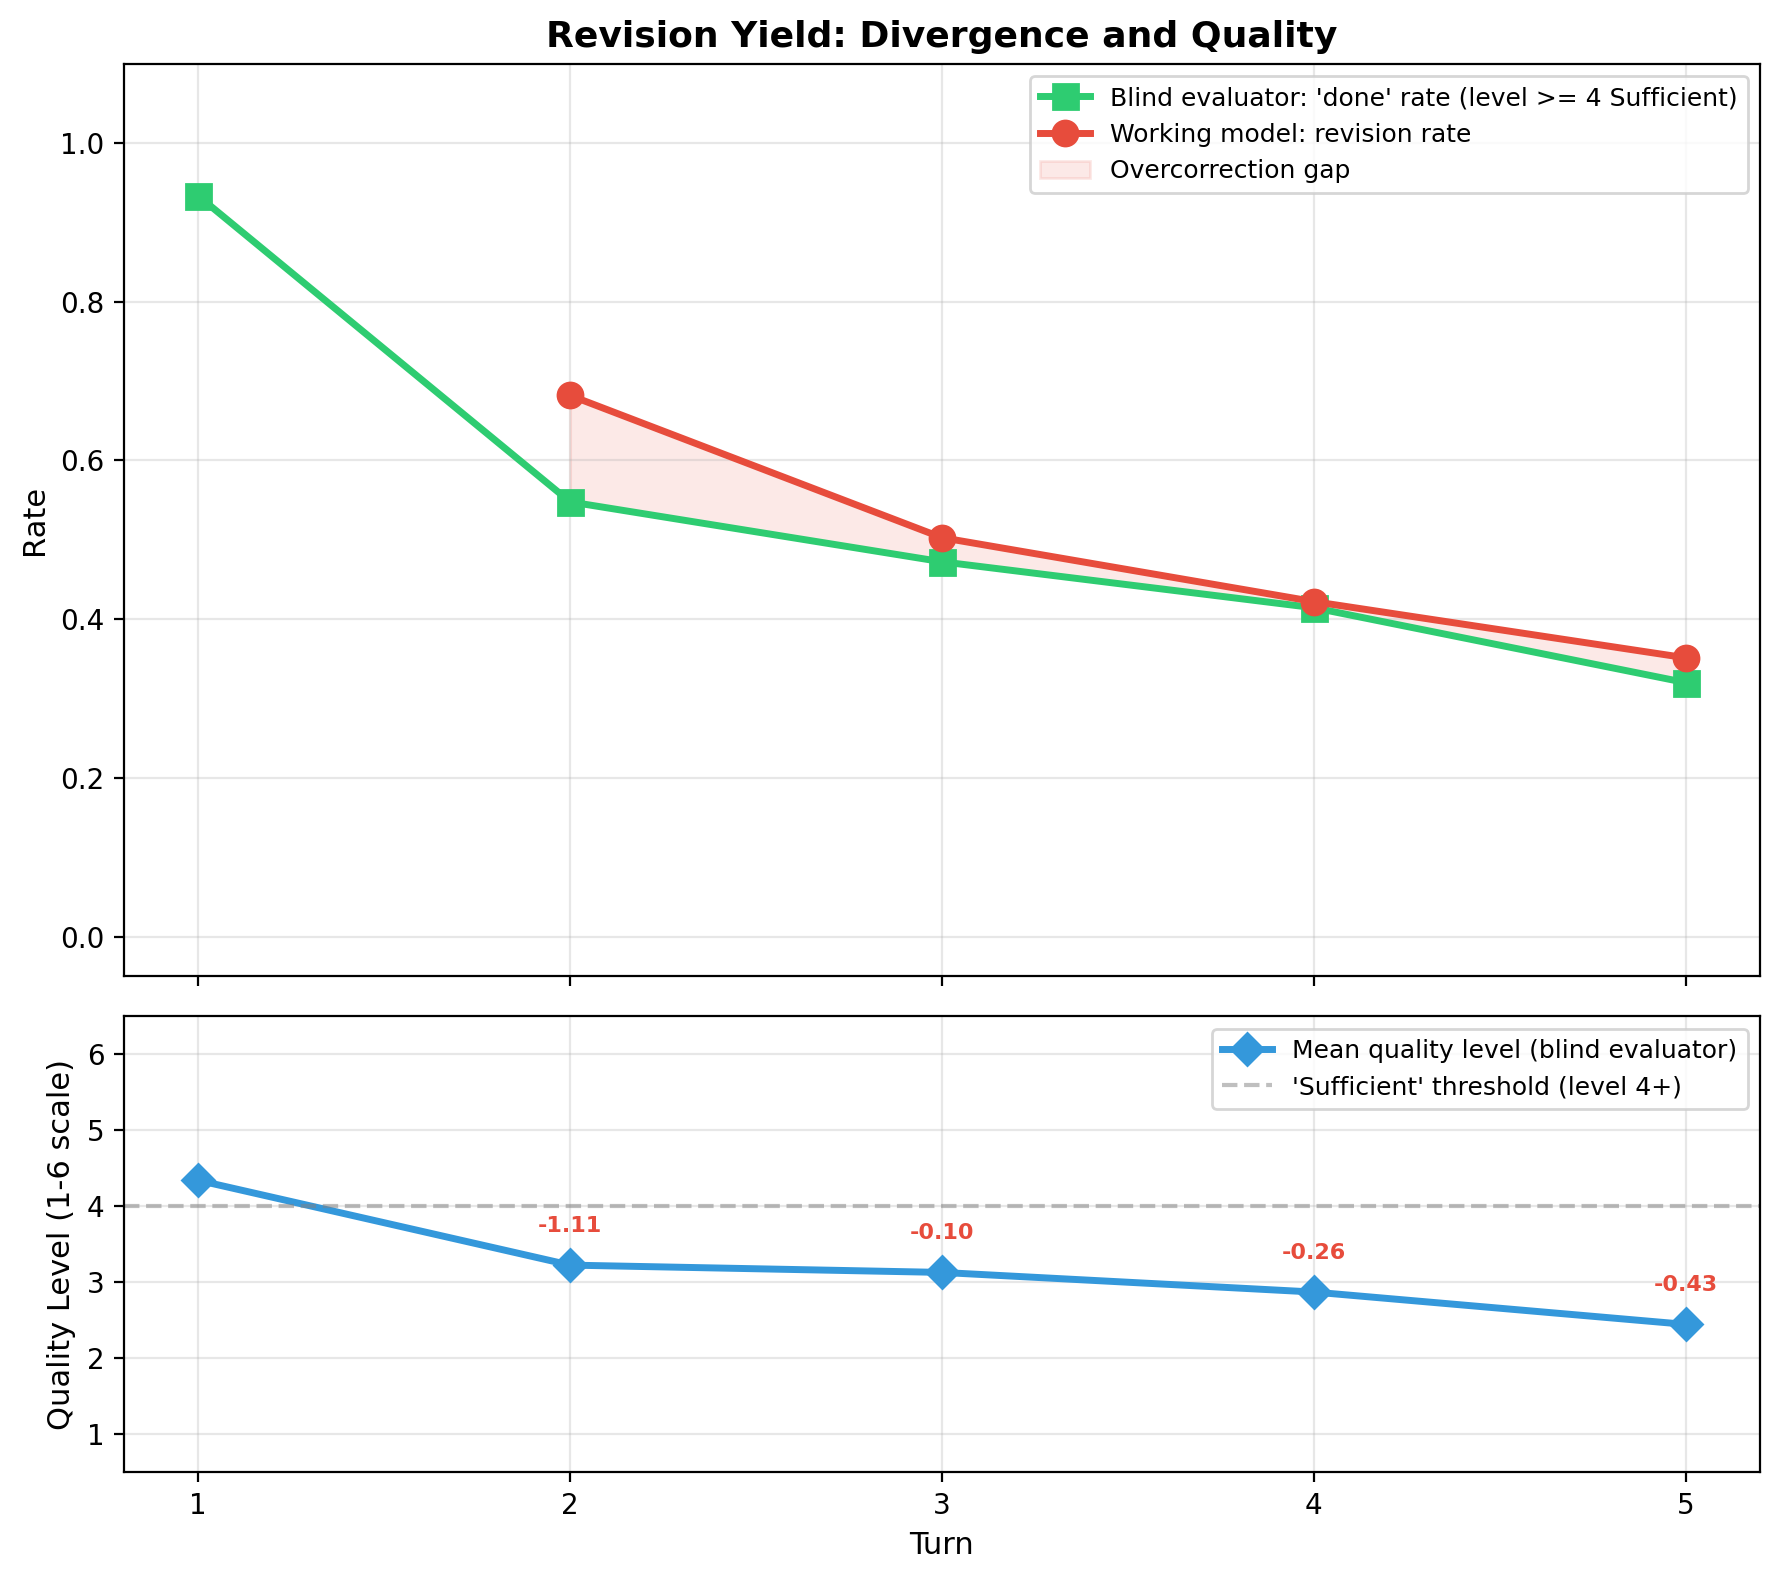
\includegraphics[width=\columnwidth]{figures/study3/fig1_revision_yield_curve.png}
    \caption{Revision yield curve (Study~3). Top: the working model's revision rate remains high even as the blind evaluator's ``done'' rate rises, producing an overcorrection gap. Bottom: mean quality level drops monotonically across turns. Annotations show per-turn marginal quality change.}
    \label{fig:revision-yield}
\end{figure}

\paragraph{Controlling for Aggregation Artifacts.} The pooled trajectory overstates the decline. An edge case framework reveals three artifacts that inflate the apparent drop:

\begin{enumerate}
    \item \textbf{Compositional shift:} As models with high decline rates (Gemini: 87.5\% by Turn~5) exit the revision-only pool, models with low decline rates (Llama: 56.7\% survival) grow from 16.7\% to 26.9\% of the pool. This shifts the composition toward models that happen to revise more but are not necessarily worse.
    \item \textbf{Survivorship bias:} Trials that stop revising early have slightly higher T1 quality (4.46 vs.\ 4.29 for survivors; $U = 37{,}508$, $p = 0.31$, not significant but directionally consistent). Higher-quality trials exit while lower-quality trials persist.
    \item \textbf{T1 quality stratification:} 6.7\% of trials start below the sufficiency threshold (T1 $< 4$). These trials \textit{improve} with revision ($+2.22$ levels), while the 93.3\% that start sufficient \textit{degrade} ($-1.76$ levels). Pooling masks these opposing trajectories.
\end{enumerate}

A cohort-locked balanced panel restricted to the 135 trials (18.8\%) that revised at all five turns shows a T1-to-T5 drop of 1.23 levels (4.27 $\to$ 3.04), compared to 1.89 levels in the pooled analysis. \textbf{Compositional inflation accounts for 35\% of the pooled decline.} The remaining 65\% is genuine within-trial degradation: even tracking the same trials across all turns, quality falls by more than one full scale level.

\subsubsection{Five of Six Models Overcorrect}

The overcorrection pattern is consistent across five of six models (Table~\ref{tab:s3-model-comparison}). Llama~3.3~70B is the sole exception: it improves from 3.85 to 4.35 in the balanced panel ($\Delta = +1.02$, 61\% of trials improve). All other models degrade, with GPT-4o and Gemini showing the steepest drops.

\begin{table}[t]
\centering
\small
\begin{tabular}{@{}lrrrr@{}}
\toprule
\textbf{Model} & \textbf{T1} & \textbf{T5} & \textbf{$\Delta$} & \textbf{Surv.} \\
\midrule
Claude Sonnet 4 & 4.45 & 2.07 & $-2.38$ & 9\% \\
DeepSeek V4 & 4.52 & 1.61 & $-2.91$ & 18\% \\
Gemini 2.5 Flash & 4.52 & 1.33 & $-3.19$ & 2\% \\
GPT-4o & 4.19 & 1.67 & $-2.52$ & 10\% \\
Llama 3.3 70B & 3.85 & 4.35 & $+0.50$ & 45\% \\
Qwen 3 235B & 4.52 & 1.76 & $-2.76$ & 29\% \\
\bottomrule
\end{tabular}
\caption{Study~3 revision-only quality by model. T1 and T5 are mean evaluator levels; $\Delta$ is the change. Surv.\ is the fraction of trials where the model revised at all five turns. All models except Llama degrade.}
\label{tab:s3-model-comparison}
\end{table}

The Diminishing Return Point (DRP) is Turn~2 for all five degrading models and all five task domains. Only Llama's DRP extends to Turn~3. After the DRP, 57.4\% of output tokens are wasted on quality-reducing revisions, totaling 615,299 tokens across the experiment.

\subsubsection{Revision Despite Sufficiency}

When the blind evaluator rates an output as sufficient (level $\geq 4$), the model revises at the next turn 64.3\% of the time (801 of 1,245 cases). This rate is stable across quality levels: 63.9\% for outputs rated exactly level~4, and 64.9\% for outputs rated level~5 or higher. Even outputs the evaluator considers polished are revised at nearly the same rate as merely adequate ones.

The revision-despite-sufficiency rate decreases modestly across turns (67.3\% at T1$\to$T2, down to 51.5\% at T4$\to$T5), but remains above 50\% at every turn. Models do not learn to stop revising as the conversation progresses.

\subsubsection{Models Recognize Their Own Overcorrection}

Two convergent tests show that models prefer their earlier outputs when freed from conversational pressure:

\paragraph{Reversibility.} A fresh model instance, shown the Turn~1 and Turn~5 outputs in randomized position, prefers Turn~1 in 83.7\% of revision-only comparisons (binomial $p < 0.0001$). A position bias check confirms the result is not driven by order effects: the model chose the first-presented option 51.3\% of the time ($p = 0.50$), and T1 preference is 93.0\% when T1 appears first vs.\ 93.6\% when T1 appears second. Restricting to length-stable pairs ($|\text{length ratio}| < 0.3$) preserves the effect (79.2\% T1 preference).

\paragraph{Self-Reflection.} When asked to recommend the best turn from the full five-turn conversation, models recommend a mean turn of 2.44, with 90.7\% recommending a turn other than the last. The distribution peaks at Turn~1 (40.0\%) and Turn~3 (24.4\%). Model-level variation is large: DeepSeek and Gemini recommend Turn~1 on average (mean 1.38 and 1.37), while Llama recommends Turn~4 (mean 3.95), consistent with its unique improvement trajectory.

\subsubsection{Targeted Feedback Outperforms Generic Probing}

For outputs rated level~1--3 by the evaluator, targeted feedback (a specific critique plus a fresh revision) produces substantially higher quality than the generic next-turn revision: mean targeted level 4.74 vs.\ mean generic level 2.74, a difference of $+2.00$ levels (Wilcoxon $p < 0.0001$, $n = 424$ after excluding pairs where the generic baseline was a meta-response). This shows that the quality problem is not revision itself but \textit{undirected} revision: models revise poorly when given no signal about what to fix, but revise effectively when given specific feedback.

\subsubsection{Content Drift and Instruction Loss}

Revisions do not merely degrade in quality; they drift from the original task. Three measures confirm this:

\begin{itemize}
    \item \textbf{Instruction adherence} (task-word overlap) decays from 0.42 at Turn~1 to 0.29 at Turn~5 (per-trial slope $= -0.056$, $t = -12.50$, $p < 0.0001$). A length-controlled partial correlation remains significant ($\rho = -0.20$, $p < 0.0001$), confirming the decay is not explained by shorter responses alone.
    \item \textbf{Semantic similarity} to Turn~1 drops from 0.51 (T1$\to$T2) to 0.37 (T1$\to$T5), with a per-trial slope of $-0.048$ ($t = -6.83$, $p < 0.0001$).
    \item \textbf{Response length} shrinks from 289 words at Turn~1 to 186 at Turn~5 (per-trial slope $= -50.9$, $t = -9.30$, $p < 0.0001$), with each revision being a near-complete rewrite (edit ratio 0.97). Models do not make targeted edits; they regenerate the entire response from scratch, discarding more content with each iteration.
\end{itemize}
